The system consists of four access layers over a single reproducible workflow runner:

\begin{itemize}
    \item CLI interface
    \item Python SDK
    \item API invocation contract
    \item Standardized external interface (Section~\ref{sec:skill})
\end{itemize}

The workflow runner executes three analysis workflows through six processing modules. The end-to-end research process is organized as a twelve-stage execution diagram (question formulation, hypothesis generation, literature retrieval, study design, data ingestion, statistical analysis, bioinformatics, output aggregation, writing, review, critique, and formatted output). Stages 1--8 are fully implemented in the current release; stages 9--12 (writing, review, critique, formatted output) describe the intended end-to-end research workflow and are not automated by the current system.

\subsection{Literature Review}
\label{sec:lit}
PubMed-based retrieval, entity extraction, co-occurrence graph construction, and research-gap identification. Outputs include a knowledge graph and a structured gap report.

\subsection{Biomarker Discovery}
\label{sec:bio}
Gene expression analysis using differential expression and pathway enrichment. Volcano plots and enriched-pathway tables are produced as reproducible outputs. Unless a real cohort is supplied, the pipeline operates on synthetic expression matrices.

\subsection{Causal Inference}
\label{sec:causal}
Mendelian randomization using simulated GWAS summary statistics. The pipeline performs inverse-variance-weighted (IVW) estimation with sensitivity analysis, producing scatter and funnel plots. All genetic inputs are simulated and explicitly labeled as such.

\begin{figure}[h]
    \centering
    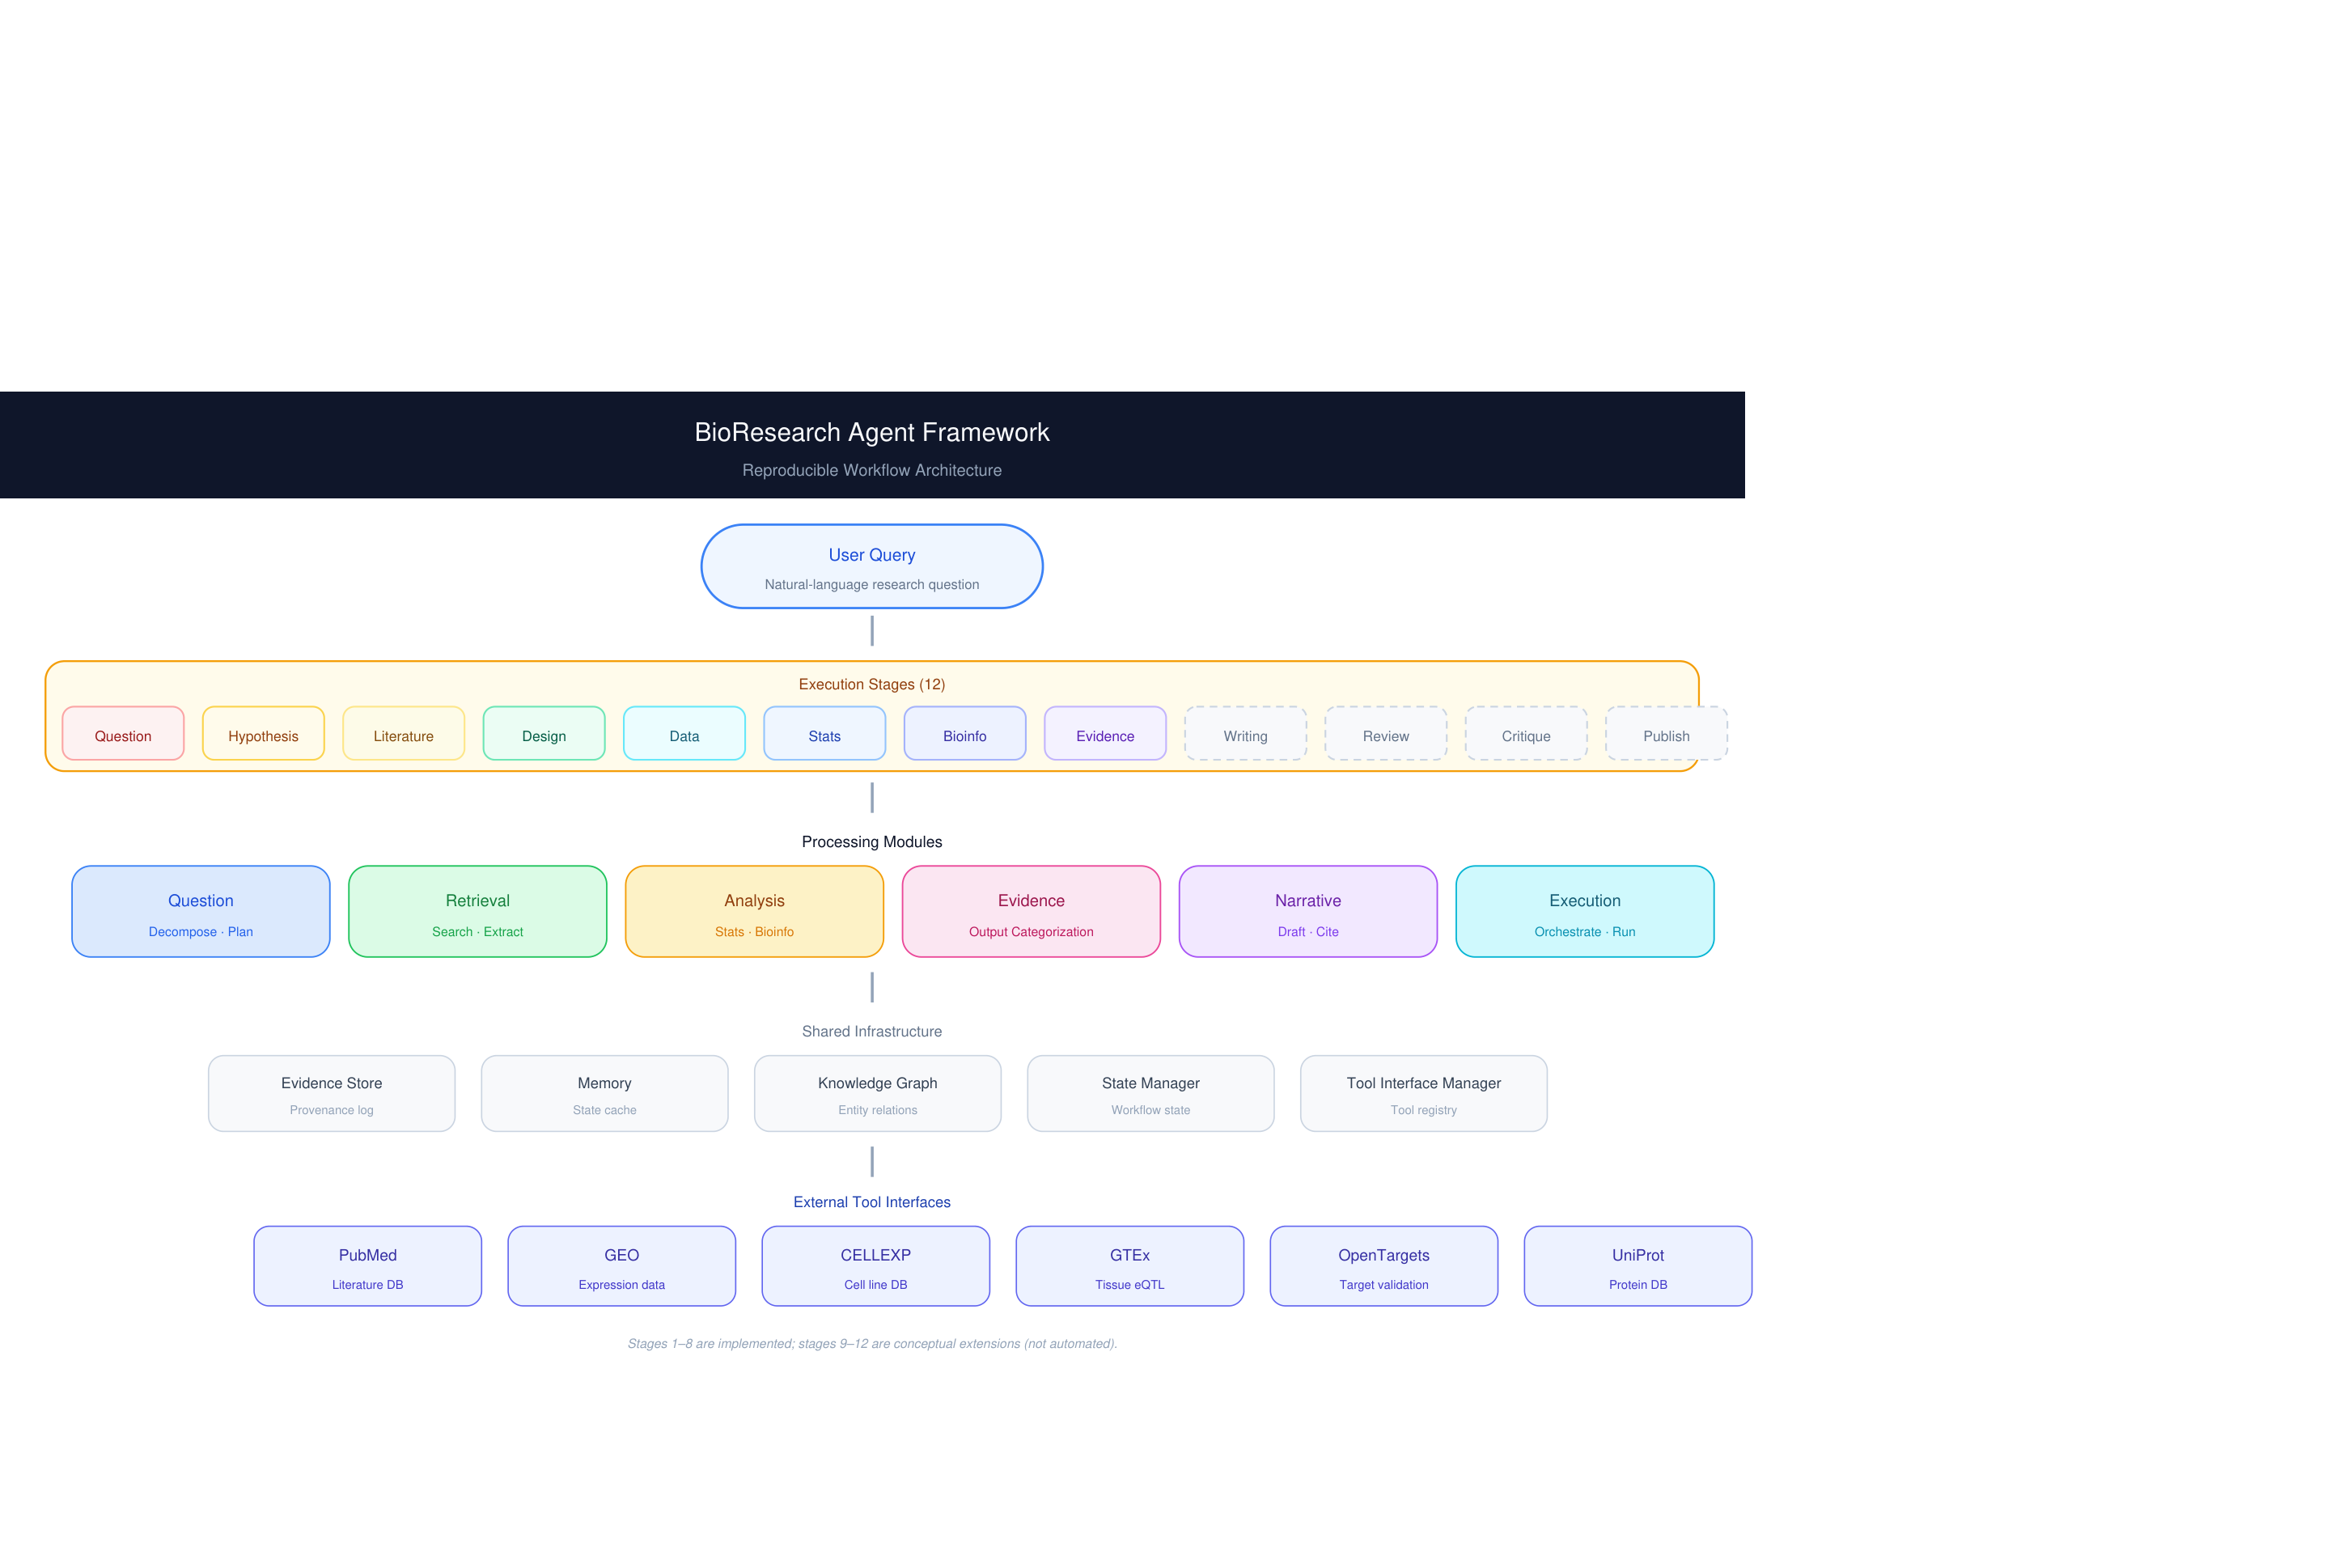
\includegraphics[width=0.9\linewidth]{figures/fig1_framework}
    \caption{System component diagram of BioResearch Agent: the workflow runner, three supported analysis pipelines, and the four access layers.}
    \label{fig:framework}
\end{figure}